% Figure: feature-oriented (MVT) vs column-oriented (MLT) layout of one layer,
% and the effect of encoding-unit size on fixed per-stream metadata.
% Requires: \usepackage{tikz}
\begin{figure*}[t]
\centering
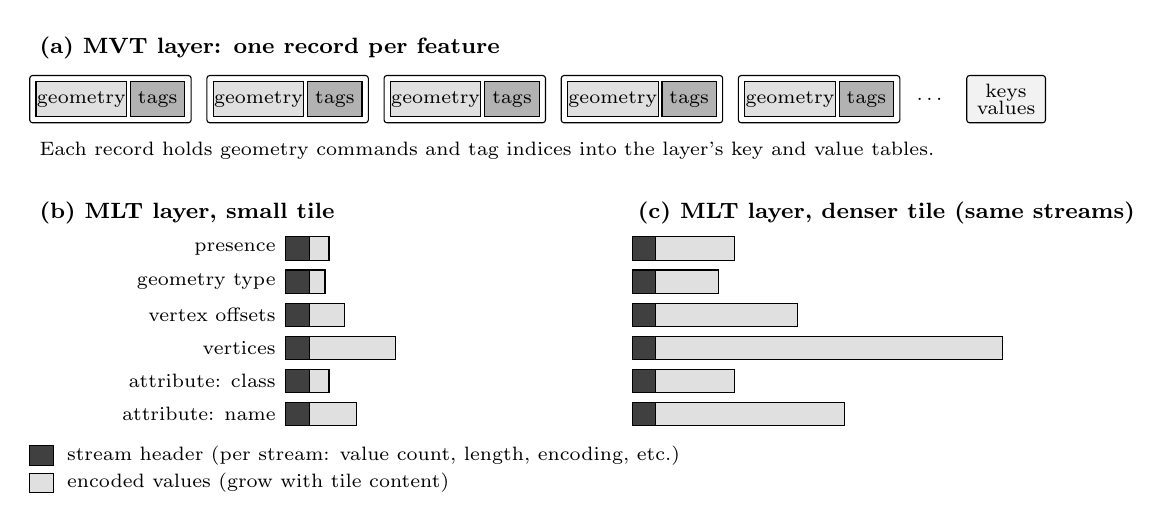
\begin{tikzpicture}[x=1cm, y=1cm, font=\scriptsize,
    hdr/.style={draw, fill=black!75, minimum height=0.32cm, inner sep=0pt},
    pay/.style={draw, fill=black!12},
    rec/.style={draw, rounded corners=1pt},
    lbl/.style={anchor=east, inner sep=2pt}]

  % ---------------- (a) MVT ----------------
  \node[anchor=west, font=\footnotesize\bfseries] at (-2.6,3.55)
        {(a) MVT layer: one record per feature};
  \foreach \i in {0,...,4} {
    \pgfmathsetmacro{\x}{-2.6+\i*2.25}
    \draw[rec] (\x,2.6) rectangle ++(2.05,0.6);
    \draw[pay] (\x+0.08,2.68) rectangle ++(1.15,0.44);
    \node at (\x+0.655,2.9) {geometry};
    \draw[draw, fill=black!30] (\x+1.28,2.68) rectangle ++(0.69,0.44);
    \node at (\x+1.625,2.9) {tags};
  }
  \node at (8.85,2.9) {\dots};
  \draw[rec, fill=black!5] (9.3,2.6) rectangle ++(1.0,0.6);
  \node[align=center] at (9.8,2.9) {keys\\[-2pt]values};
  \node[anchor=west] at (-2.6,2.25)
        {Each record holds geometry commands and tag indices into the layer's key and value tables.};

  % ---------------- (b) MLT, small tile ----------------
  \node[anchor=west, font=\footnotesize\bfseries] at (-2.6,1.45)
        {(b) MLT layer, small tile};
  \node[anchor=west, font=\footnotesize\bfseries] at (5.0,1.45)
        {(c) MLT layer, denser tile (same streams)};

  \def\names{{"presence","geometry type","vertex offsets","vertices","attribute: class","attribute: name"}}
  \def\small{{0.25,0.20,0.45,1.10,0.25,0.60}}
  \foreach \k in {0,...,5} {
    \pgfmathsetmacro{\y}{1.0-\k*0.42}
    \pgfmathparse{\names[\k]}\edef\nm{\pgfmathresult}
    \pgfmathsetmacro{\w}{\small[\k]}
    \pgfmathsetmacro{\W}{min(4*\small[\k],4.6)}
    % small tile
    \node[lbl] at (0.6,\y) {\nm};
    \draw[fill=black!75] (0.65,\y-0.15) rectangle ++(0.3,0.30);
    \draw[pay] (0.95,\y-0.15) rectangle ++(\w,0.30);
    % dense tile
    \draw[fill=black!75] (5.05,\y-0.15) rectangle ++(0.3,0.30);
    \draw[pay] (5.35,\y-0.15) rectangle ++(\W,0.30);
  }

  % legend
  \draw[fill=black!75] (-2.6,-1.75) rectangle ++(0.3,0.25);
  \node[anchor=west] at (-2.25,-1.625) {stream header (per stream: value count, length, encoding, etc.)};
  \draw[pay] (-2.6,-2.1) rectangle ++(0.3,0.25);
  \node[anchor=west] at (-2.25,-1.975) {encoded values (grow with tile content)};
\end{tikzpicture}
\caption{Feature-oriented and column-oriented layouts of one tile layer.
(a)~MVT stores a sequence of feature records.
(b)~MLT stores each property of all features as a column, split into streams of same-typed values;
every stream carries a header.
(c)~When a spatial encoding unit holds more content, streams become longer, amortizing per-stream
headers and exposing longer value sequences to lightweight encodings. MLT also contains layer- and
column-level structural bytes not drawn here; Section~\ref{sec:results-streams} reports total
non-payload structural share separately from stream-header share. Proportions are schematic.}
\label{fig:mvt-mlt-streams}
\end{figure*}